\section{Gameplay}

The game will be made using Unity. Movement and jumping will be implemented using Unity's 2D physics engine to handle.

\begin{figure}[ht]
\centering
\begin{subfigure}{.5\textwidth}
  \centering
  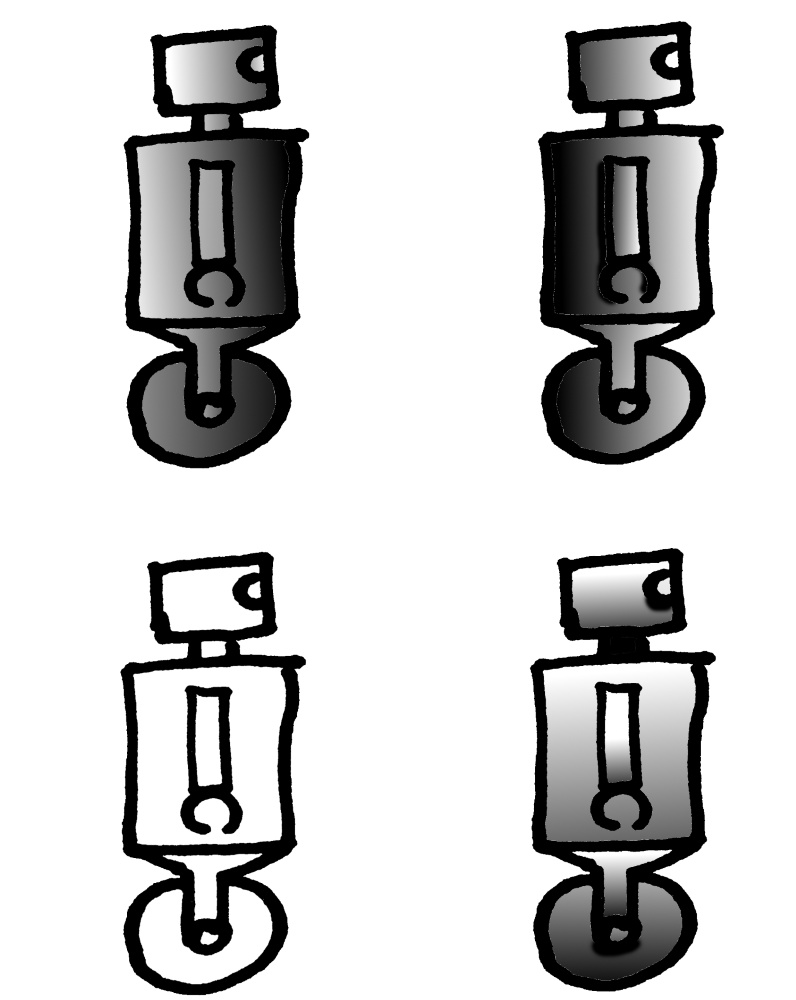
\includegraphics[scale=0.2, trim = 0cm 0cm 0cm 2cm]{images/in}
  \caption{input files including a base file and the same file drawn as if it was lit from a handful of different directions}
  \label{fig:sub1:pl}
\end{subfigure}%
\begin{subfigure}{.5\textwidth}
  \centering
  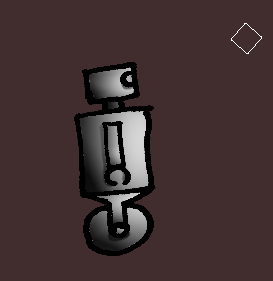
\includegraphics[scale=0.9, trim = 0cm 0cm 0cm 0.5cm]{images/out}	
  \caption{output file reacting to a dynamic light shown by the white cube}
  \label{fig:sub2:pl}
\end{subfigure}
\caption{Player character mock-up}
\label{fig:player}
\end{figure}

Re-activating components of the ship has a probability of activating some of the ship's security measures. These will include activating traps or spawning hostile defence drones. On reaching the next component these security systems can be deactivated.



We plan to use 2d sprites, with normal maps created using \textit{SpriteLamp} for the game's lighting effects. Figure~\ref{fig:player} shows an example of it's use.